\section{Process Analysis}
Usually, in this type of exercises, you are given a process model, enriched with branching probabilities, along with
a table containing the cycle time and processing time measures for each activity.
\subsection{Quantitative Analysis}
\begin{exercise}{1}
\begin{figure}[H]
    \centering
    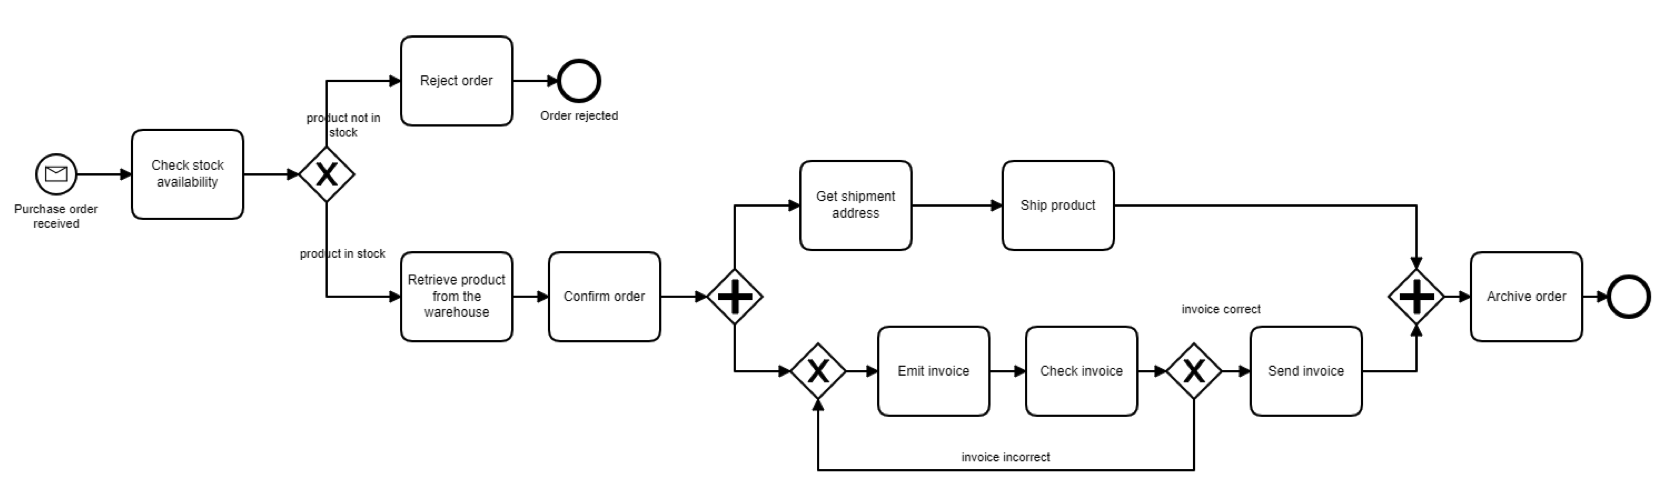
\includegraphics[width=\textwidth]{images/exercises/q_a_bpnm.png}
    \caption{Example Process for Quantitative Analysis Exercises}
\end{figure}
\begin{itemize}
    \item 20\% of the orders are rejected for product not in stock;
    \item 10\% of the orders have an incorrect invoice;
\end{itemize}
and the following table:
\begin{table}[H]
    \centering
    \resizebox{0.8\textwidth}{!}{%
        \begin{tabular}{c|c|c}
            \hline
            \textbf{Activity} & \textbf{Cycle Time (CT)} & \textbf{Processing Time (PT)} \\
            \hline
            Check stock availability & 1 day & 30 min \\
            Reject order & 7 days & 1 hour \\
            Retrieve product from the warehouse & 3 days & 4 hours \\
            Confirm order & 4 days & 2 hours \\
            Get shipment address & 1 day & 30 min \\
            Ship product & 10 days & 24 hours \\
            Emit invoice & 1 day & 1 hour \\
            Check invoice & 1 day & 30 min \\
            Send invoice & 2 days & 30 min \\
            Archive order & 4 days & 1 hour \\
            \hline
        \end{tabular}
    }
\end{table}
Using the information provided, compute the following:
\begin{enumerate}
    \item The \textbf{Cycle Throughput Time} of the process;
    \item The \textbf{Cycle Time} of the process;
    \item The \textbf{Cycle Time Efficiency (CTE)} of the process;
\end{enumerate}
\end{exercise}
\paragraph{Solution:}
\begin{enumerate}
    \item The Cycle Throughput Time can be computed with the rules provided in the \ref{fig:cycle_time_table}. The resulting equation is:
    \[CT = 1 + (7 \times 0.2) + \left[\left(3 + 4 + \max\left(1 + 10, \frac{(1 + 1)}{0.9} + 2\right) + 4 \right) \times0.8\right]\]
    \[ = 1+ 1.4 + \left[(3 + 4 + 11 + 4) \times 0.8\right] = 2.4 + 17.6 = 20 \text{ days}\]
    \item The Processing Time can be computed similarly, simply substituting the cycle times with processing times:
    \[PT = 0.5 + (1 \times 0.2) + \left[\left(4 + 2 + \max\left(0.5 + 24, \frac{(1 + 0.5)}{0.9} + 0.5\right) + 1 \right) \times0.8\right]\]
    \[ = 0.5 + 0.2 + \left[(4 + 2 + 24.5 + 1) \times 0.8\right] = 0.7 + 6 \times 0.8 = 0.7 + 25.2 = 25.9 \text{ hours}\]
    \item Finally, we can compute the Cycle Time Efficiency as:
    \[CTE = \frac{PT}{CT} = \frac{25.9 \text{ hours}}{20 \text{ days}} = \frac{25.9}{20 \times 8} = 16\%\]
\end{enumerate}
\subsection{Work In Progress (WIP) Analysis}
\begin{exercise}{1}
Suppose that a fast food restaurant processes on average 1200 customers per day, between 10:00 and 22:00 (12 hours).
During peak hours (6 hrs per day), the restaurant receives around 900 customers in total and 90 customers (WIP) can be found waiting in line.
At non peak times, the restaurant receives 300 customers in total and 30 customers (WIP) can be found waiting in line.
\begin{enumerate}
    \item Calculate the average time that a customer spends in the restaurant during peak hours (cycle time);
    \item Calculate the average time that a customer spends in the restaurant during non-peak hours;
    \item Knowing that the restaurant expects to have more customers during peak hours, and the restaurant capacity is limited, what can the restaurant do to address this?
\end{enumerate}
\end{exercise}
\paragraph{Solution:}
Using Little's Law, we can calculate the cycle time as:
\begin{equation*}
    CT_{\text{peak}} = \frac{WIP_{\text{peak}}}{\lambda_{\text{peak}}} = \frac{90 \text{ customers}}{900 \text{ customers} / 6 \text{ hours}} = 0.6 \text{ hours} = 36 \text{ minutes}
\end{equation*}
Using the same formula, we can calculate the cycle time during non-peak hours:
\begin{equation*}
    CT_{\text{non-peak}} = \frac{WIP_{\text{non-peak}}}{\lambda_{\text{non-peak}}} = \frac{30 \text{ customers}}{300 \text{ customers} / 6 \text{ hours}} = 0.6 \text{ hours} = 36 \text{ minutes}
\end{equation*}
Since we expect more customers during peak hours (higher arrival rate), but the WIP cannot increase, the only way to keep the cycle time constant
is to decrease the cycle time during peak hours, for example by increasing the number of staff during peak hours, or optimizing the process to serve customers faster.